\glsresetall
\chapter{Background and Literature Review} \label{ch:LR}
In this chapter, the necessary background for radar theory and radar-based vital sign monitoring is first provided for a better understanding of the proposed methods in the later chapters. In addition, representative signal processing and deep learning methods for cardiac feature extraction are also introduced to provide a comprehensive review of the development over the last decade.

\section{Background Knowledge}
\subsection{Radar Types}
Different radar systems transmit different types of waveforms as shown in Figure~\ref{fig:intro_overall}(b). For example, \gls{cw} radar uses continuous wave with a fixed frequency, FMCW radar uses continuous wave with linearly increased frequency, and \gls{uwb} radar uses pulses with wide frequency bandwidth. The phase components of the transmitted signals for CW and FMCW radar are modulated by the displacement composed by respiration, heartbeat and all kinds of noises in a non-linear manner as proved in~\cite{chen2021movi,li2013review}. Then, the phase variation hidden in the raw received signal can be revealed using phase unwrapping techniques such as arctangent demodulation and extended differentiate and cross-multiply algorithm~\cite{obadi2021survey,wang2020remote}. For IR-UWB radar, the cardiac features are embedded in the propagation time delay of the echo signal~\cite{obadi2021survey}. 

Different radar types require different architectures and are suitable for different tasks. For example, CW radar has a simple architecture and adopts the fundamental baseband signal-processing methods, but the range information cannot be extracted from the received signals due to the lack of modulation~\cite{singh2020multi}. FMCW radar outperforms CW radar by leveraging the frequency modulation techniques, improving the \gls{snr} and providing the capability of range detection to further isolate the signal reflected only from the chest region~\cite{ha2020contactless}. Different from the continuous waveform used in CW and FMCW radar, IR-UWB radar emits widely spaced pulses with very short duration (e.g., $0.1-2$ ns)~\cite{hirt2003ultra}. Therefore, IR-UWB radar is more power-efficient than FMCW radar but normally cannot ensure a high SNR and range resolution~\cite{obadi2021survey}. In literature, IR-UWB radar is normally used for through-the-wall or long-distance monitoring~\cite{shen2018respiration}, but the complex radar architecture (e.g., requiring internal delay calibration~\cite{singh2020multi}) and signal-processing algorithms (e.g., harmonic rejection~\cite{wang2020experimental}) limit the relative research\cite{li2013review}.
        
In addition to the different radar types, radar operating frequency (carrier frequency) is another crucial parameter affecting cardiac monitoring quality because the frequency is inversely related to the beamwidth for antennas with the same diameter~\cite{huang2021antennas}, enabling the radar system with high operating frequency using narrow beamwidth to enhance directivity~\cite{ramasubramanian2018moving}.  Obeid \textit{et al.}~\cite{obeid2008low} found out that high operating frequency provides a large phase difference caused by heart vibration and improves the sensitivity of cardiac monitoring. The researchers in~\cite{ramasubramanian2018moving} claimed that the radar with a high operating frequency, especially the mmWave range ($30-300$ GHz), can achieve a high range resolution, good noise-robustness and small antenna size.

According to the review of the trends in radar usage for the recent decade, CW radar was the most popular type before 2020 due to its simple architecture; FMCW radar receives a growing concern since 2015 because the recent-released commercial FMCW radar platforms reduce the knowledge required for designing or setting up a radar system~\cite{zhou2022towards}; IR-UWB radar is less popular than the other two types due to its complex radar architecture and signal-processing algorithms~\cite{singh2020multi,wang2020experimental}. For the trend in operating frequency selection, early studies all focus on the low-frequency band for the simplicity of radar architecture design and baseband signal-processing algorithms, whereas the recent researchers are steering toward using mmWave radar (especially $60$ or $77$ GHz commercial radar platform) for good performance. In summary, the FMCW with high operating frequency is becoming the mainstream for radar-based cardiac monitoring due to the balance between the performance and complexity, and the complexity for settling the radar platform is also significantly reduced due to the emergency of commercial radar.

\subsection{Theoretical Background for Vital Sign Monitoring}
\subsubsection{Cardiac Signal Extraction from CW Radar}
The vanilla signal model for radar-based cardiac monitoring (e.g., heart rate monitoring) using CW radar starts from the transmitted signal expressed as
\begin{equation}
s_t(t)=A_t\cdot\cos (2 \pi f t+\theta(t))
\end{equation}
where $A_t$ and $f$ are the amplitude and carrier frequency of the transmitted signal, and $\theta(t)$ is the phase noise from the signal generator with respect to time $t$~\cite{droitcour2004range}. In the ideal case, the radar signal is only reflected by a human at a fixed distance $d_0$ with a varying chest displacement as $x(t)$, and the received signal after propagation time $T_p(t)$ can be derived as
\begin{equation}
s_r(t)=A_r\cdot\cos (2 \pi f (t-T_p(t))+\theta(t-T_p(t)))
\end{equation}
with
\begin{equation}
\begin{aligned}
T_p(t) &= \frac{2d(t)}{c} \\
d(t) &= d_0+x(t)
 \end{aligned}
\end{equation}
where $A_r$ is the amplitude of the received signal, $c$ is the light speed and $2d(t)$ represents the round trip distance of the signal between the transmitter and receiver. Then, the received signal can be expanded as
\begin{equation}
s_r(t)=A_r\cdot\cos (2 \pi ft-\frac{4\pi d_0}{\lambda}-\frac{4\pi x(t)}{\lambda}+\theta(t-\frac{2 d_0}{c}-\frac{2 x(t)}{c}))
\end{equation}
where $\lambda$ is the wavelength that equals to $\frac{c}{f}$. According to~\cite{droitcour2004range,lin2022broadband}, it is safe to eliminate changes in amplitude and phase noise term because the chest displacement is much less than the fixed distance (i.e., $x(t)\ll d_0$). Therefore, the approximate received signal is
\begin{equation}
s_r(t)\approx \cos (2 \pi ft-\frac{4\pi d_0}{\lambda}-\frac{4\pi x(t)}{\lambda}+\theta(t-\frac{2 d_0}{c}))
\end{equation}

The received signal $s_r(t)$ will then pass a local oscillator with a low-pass filter to remove the frequency term, and the resultant baseband signal is
\begin{equation}
s_b(t)=cos(\theta_d+\frac{4\pi x(t)}{\lambda}+\Delta \theta(t))
\end{equation}
with
\begin{equation}
\begin{aligned}
 \theta_d &= \frac{4\pi d_0}{\lambda} + \theta_{0}\\
\Delta \theta (t) &= \theta(t)- \theta(t-\frac{2 d_0}{c})
 \end{aligned}
\end{equation}
where $\theta_d$, $\theta_0$ and $\Delta \theta (t)$ are phase shifts affected by different factors such as $d_0$, signal mixer and antenna, and can be set as constant~\cite{lin2022broadband}. Then, the phase signal unwrapped from the baseband signal is obtained as
\begin{equation}
\phi(t) = \theta_d+\frac{4\pi x(t)}{\lambda}+\Delta \theta(t)
\end{equation}

Finally, the vanilla signal model derived above shows that the chest displacement $x(t)$ is involved in the phase variation of the baseband signal as
\begin{equation}\label{equ:phase1}
\Delta\phi(t) = \frac{4\pi x(t)}{\lambda}
\end{equation}

The follow-up researchers have proposed various techniques to improve the accuracy of the unwrapped phase signal variation in (\ref{equ:phase1}). For example, the in-phase/quadrature modulation is proposed to solve the null point issue~\cite{droitcour2004range}; the differentiate and cross-multiply algorithm is designed to avoid discontinuity in the unwrapped phase signal~\cite{zhang2023overview}. In addition, chest displacement $x(t)$ is a mixture of cardiac activities, respiration and noises (e.g., \gls{rbm}~\cite{chen2021movi,zhang2020health}, multi-path or multi-person interference~\cite{mercuri2021enabling,islam2022contactless}). Therefore, enormous advanced algorithms are proposed to decompose cardiac information from $x(t)$, as have been reviewed in~\cite{zhang2023overview}.

\subsubsection{Cardiac Signal Extraction from FMCW Radar}
FMCW could provide advanced features that allows the extraction of the signal reflected from certain points. In the literature, FMCW radar has been widely used in nowadays \gls{mmWave} sensing to measure the range, velocity and \gls{aoa} of the objects appearing in the field of view~\cite{tang2024bsense}, with three critical concepts that configure the transmitted waveform:
\begin{itemize}
\item \textbf{Chirp } is the minimum component in the FMCW signal with microsecond-level duration and is often called fast time. The waveform of a single chirp is a sinusoidal signal with frequency that changes linearly over time, with the key characteristics designated by start frequency, bandwidth and chirp duration to get range information of the object.
\item \textbf{Frame} is a collection of multiple chirps that forms a complete observation window to get the velocity information based on the range bins extracted from chirps and is often referred to as slow time.
\item \textbf{Virtual antenna array (channel)} is a commonly used concept in \gls{mimo} radar systems and is able to realize complex modulations or beamforming~\cite{xiong2022vital}. However, this study mainly leverages the phase difference across antenna channels to estimate the AoA of the objects.
\end{itemize}
The popular commercial radar platforms have provided a convenient interface for radar configuration, signal modulation and demodulation~\cite{AWR1843}, and the reflected signal from a give point $E=(x,y,z)$ in 3D space can be expressed as:
\begin{equation}\label{equ:raw_sig}
R(E, t)=\sum_{v=1}^V \sum_{c=1}^C \sum_{n=1}^N s_{v, c, n}(t)\cdot e^{j 2 \pi \frac{2k\cdot d(E, v)}{\text{light speed}} n} \underbrace{e^{j 2 \pi \frac{2\cdot d(E, v)}{\lambda}}}_{\text{phase term}\ \phi}
\end{equation}
where $(x,y,z)$ represents the (horizontal, radial, vertical) axis, $V$ is the number of virtual antenna channels, $C$ means the number of chirps within one frame, $N$ is the total sample points within one chirp, $s_{v, c, n}(t)$ denotes the original received signal, $k$ is the slope of frequency raising, $\lambda$ means wavelength and $d(E, v)$ represents the distance between point $E$ and virtual antenna $v$~\cite{chen2022contactless}. In FMCW processing for vital sign monitoring, the time sample $t$ corresponds to one frame instead of the sample point $n$, and the signal from different chirps $c$ and antenna channels $v$ will be accumulated to improve SNR~\cite{liu2024diversity}.

The interested term in (\ref{equ:raw_sig}) is the variation of distance $d(E,v)$, because it represents the displacements caused by respiration and heartbeat (without considering any other noise). Therefore, the chest region displacement $h(E, t)$ can be unwrapped from phase variation $\Delta \phi$ as
\begin{equation}\label{equ:phase}
h(E, t) = \frac{\lambda \Delta \phi}{4\pi}
\end{equation}

At last, some common noises, such as respiration and thermal noise, can be easily removed using a band-pass filter and differentiator to make sure that the final $h(E, t)$ mostly contains cardiac-related features from point $E$. 

\subsection{Radar-Based ECG Monitoring as a Domain Transformation Problem}
Coarse cardiac monitoring only aims to detect a single heartbeat within one cardiac cycle, while fine-grained cardiac monitoring requires recovering subtle cardiac activities within one cardiac cycle. For example, Figure~\ref{fig:scg_ecg} shows the typical radar and SCG signal waveform within a single cardiac cycle that describes the cardiac mechanical activities, such as aortic valve opening/closure (AO/AC) and mitral valve opening/closure (MO/MC)~\cite{swift2021stop,orkand1964heart}. These mechanical activities are muscle contractions stimulated by cardiac electrical events, such as P-wave, QRS-complex and P-wave in the ECG signal as shown in Figure~\ref{fig:scg_ecg}. Therefore, radar-based ECG recovery is actually a domain transformation problem that translates cardiac mechanical activities into electrical activities and realizes fine-grained vital sign monitoring in a contactless manner.
 \begin{figure}[tb] 
    \centering 
    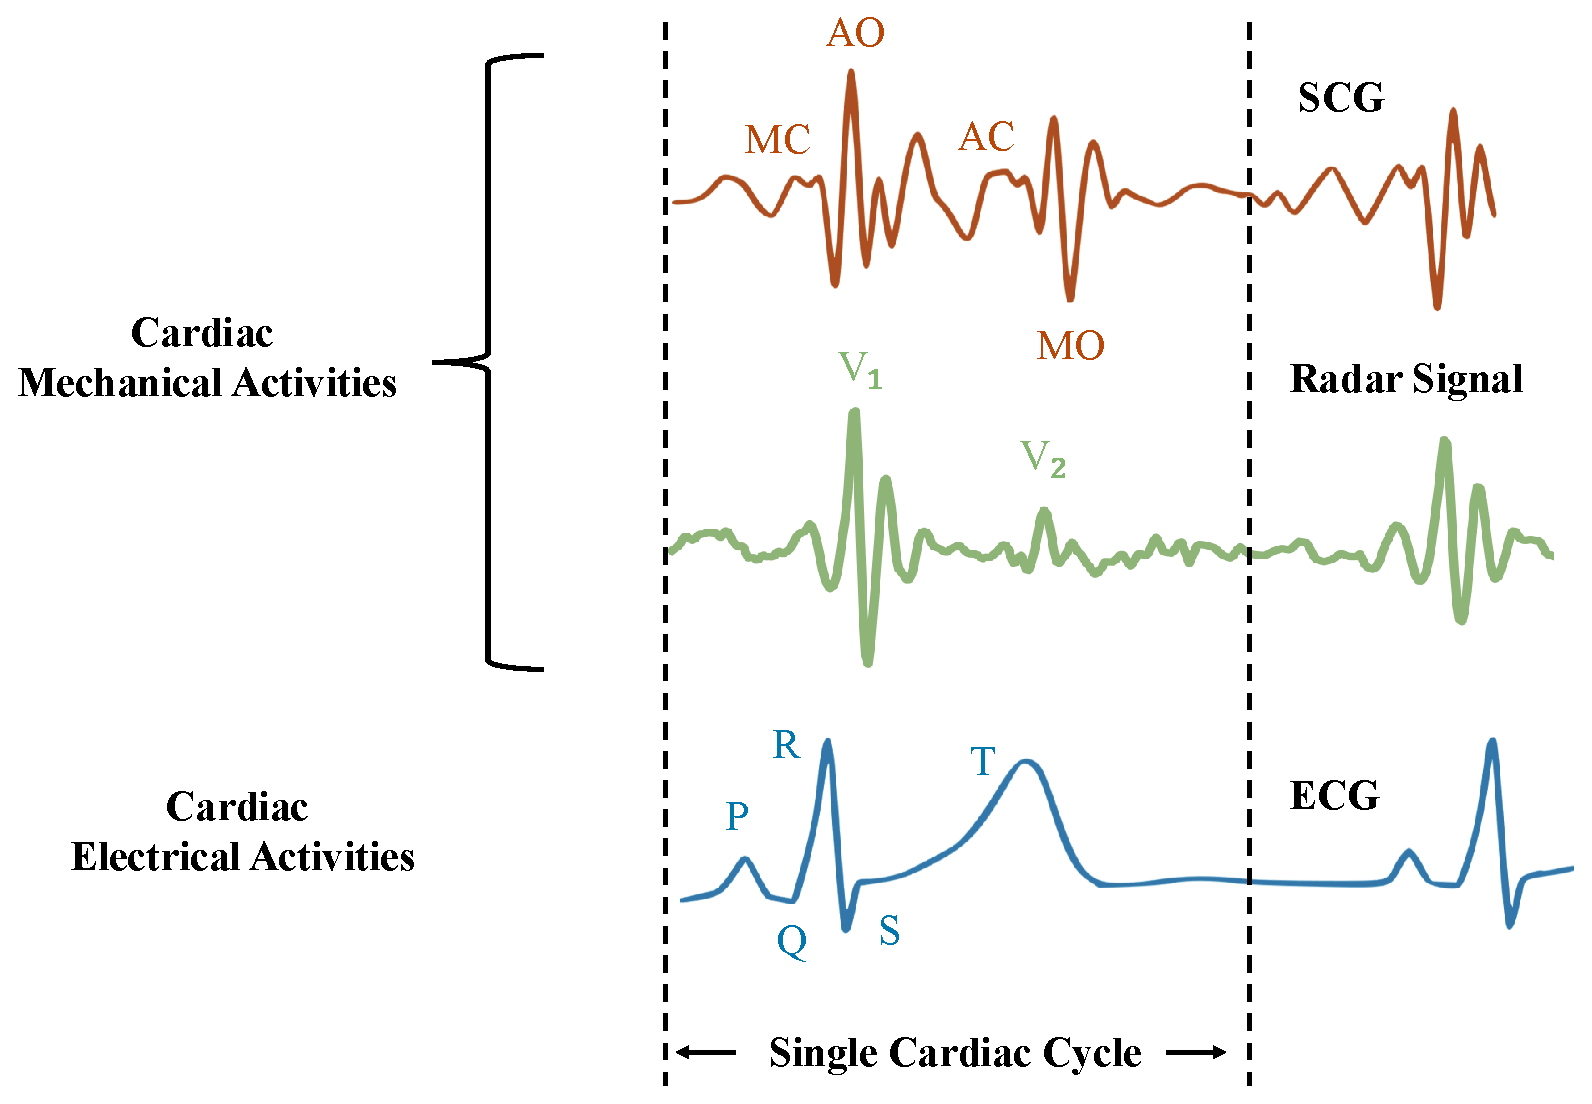
\includegraphics[width=0.8\columnwidth]{scg_ecg.eps}
    \caption{Relationships between cardiac mechanical and electrical activities within the same cardiac cycle.} 
    \label{fig:scg_ecg} 
\end{figure}
In the literature, the domain transformation is only realized by deep-learning-based methods, while a common issue of the deep learning model is not robust against large-scale noise (e.g., RBM) as reported by many previous studies~\cite{wu2023contactless,li2024radarnet,wang2023ecg,zhao2024airecg}. However, there is no existing work that investigates the noise-robustness of the deep learning model itself, and this thesis is motivated to develop a noise-robust deep learning model to realize the domain transformation in the presence of body movement noise.

\section{Literature Review for Cardiac Feature Extraction}
\subsection{Spectrum-based Methods}
Spectrum represents the transformation of signal from time-domain to frequency-domain and can reveal the main frequency components of the signal~\cite{petrovic2019high, saluja2019supervised, yang2020vital, zhu2018fundamental, le2020heartbeat, zhao2016emotion, xiong2020differential, hu2014real, xiong2017accurate, tu2015fast, park2017polyphase, shih2021quadrature, tomii2015heartbeat, li2017wavelet, mercuri2019vital, wang2020remote, liu2022vital, ling2022non}. Normally, the \gls{rr}) and HR frequency at rest are in the range of $0.1-0.5$ Hz and $1-1.6$ Hz respectively~\cite{mogi2017heartbeat}, making the spectrum-based method the most straightforward way to extract cardiac features within a certain frequency range. The spectrum-based methods usually share similar ideas: (a) a piece of unwrapped phase signal taken from the dataset only shows the periodic displacement induced by strong respiration instead of subtle cardiac activities as shown in Figure~\ref{fig:rawRadar}; (b) the raw signal is then transformed into a spectrum using time-frequency transformation methods (e.g., \gls{fft}, \gls{cwt}) as shown in Figure~\ref{fig:rawRadar_fft} with corresponding peaks labelled; (c) for the low-noise scenario, after filtering the frequency components of RR, RR harmonic and other high-frequency noise, the remaining dominant peak of the spectrum represents the HR frequency; (d) for the noisy scenario, the researchers could use several techniques, such as noise-cancellation filter or differentiator, to suppress the noise or enhance the HR frequency component on the spectrum.

\begin{figure}[tbp]
    \centering
    \subfloat[]{\label{fig:rawRadar}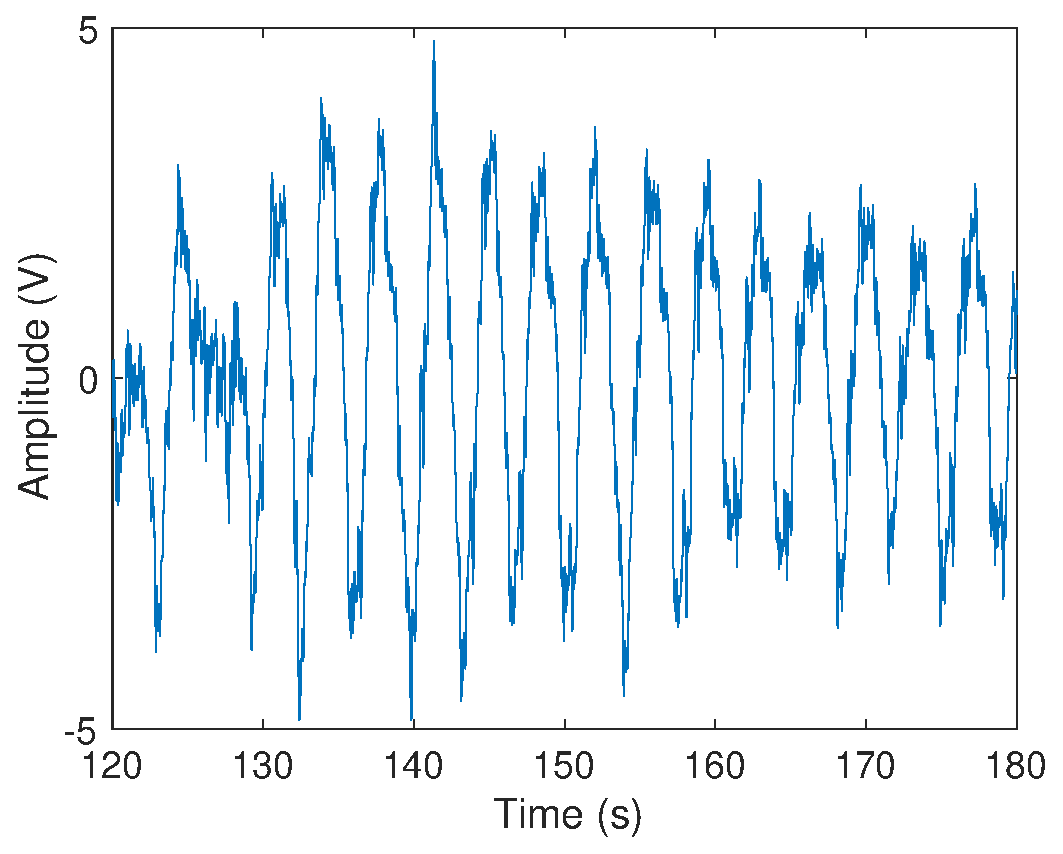
\includegraphics[width=0.25\columnwidth]{raw.eps}}
    \subfloat[]{\label{fig:rawRadar_fft}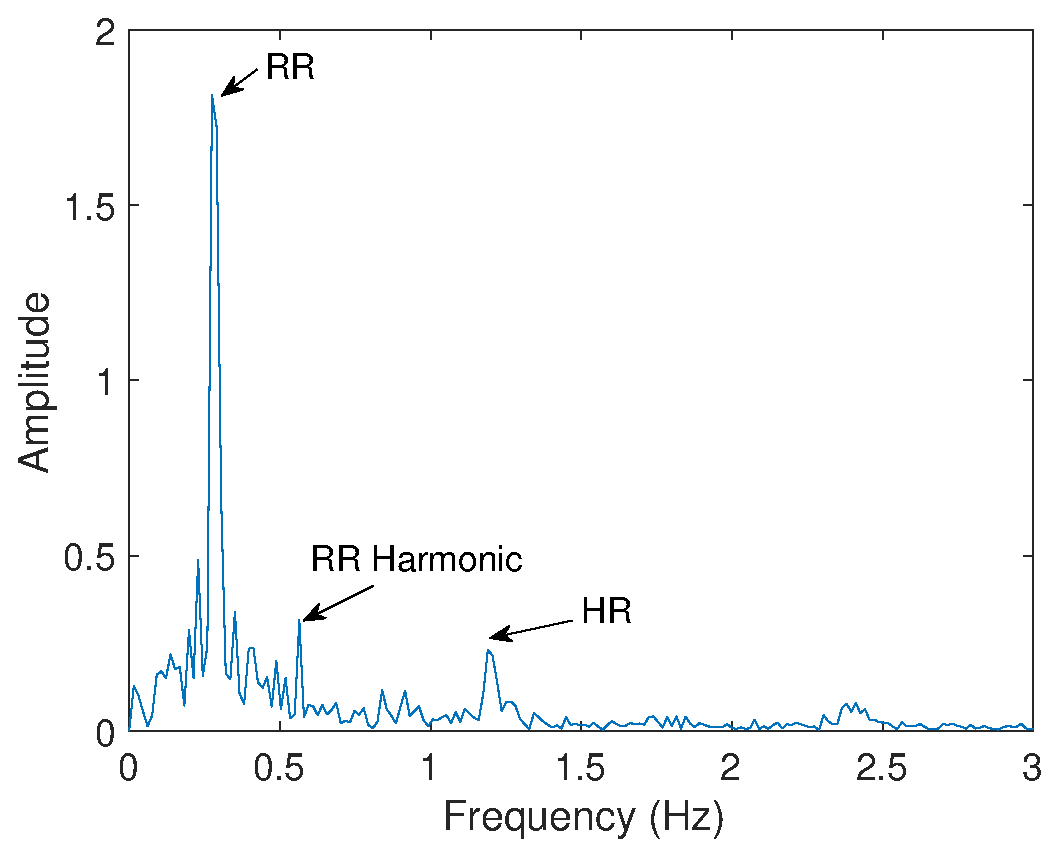
\includegraphics[width=0.25\columnwidth]{fft.eps}} 
    \subfloat[]{\label{fig:rawRadar_diff}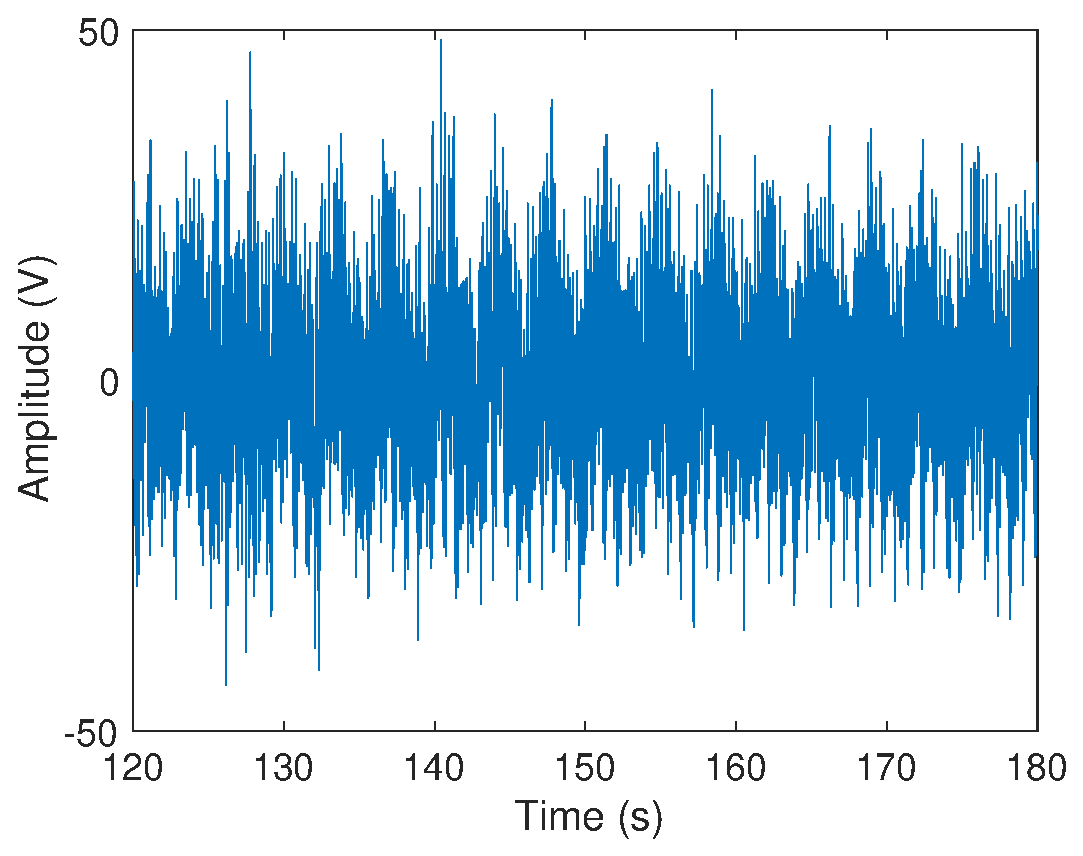
\includegraphics[width=0.25\columnwidth]{rawRadar_diff.eps}}
    \subfloat[]{\label{fig:rawRadar_diff_fft}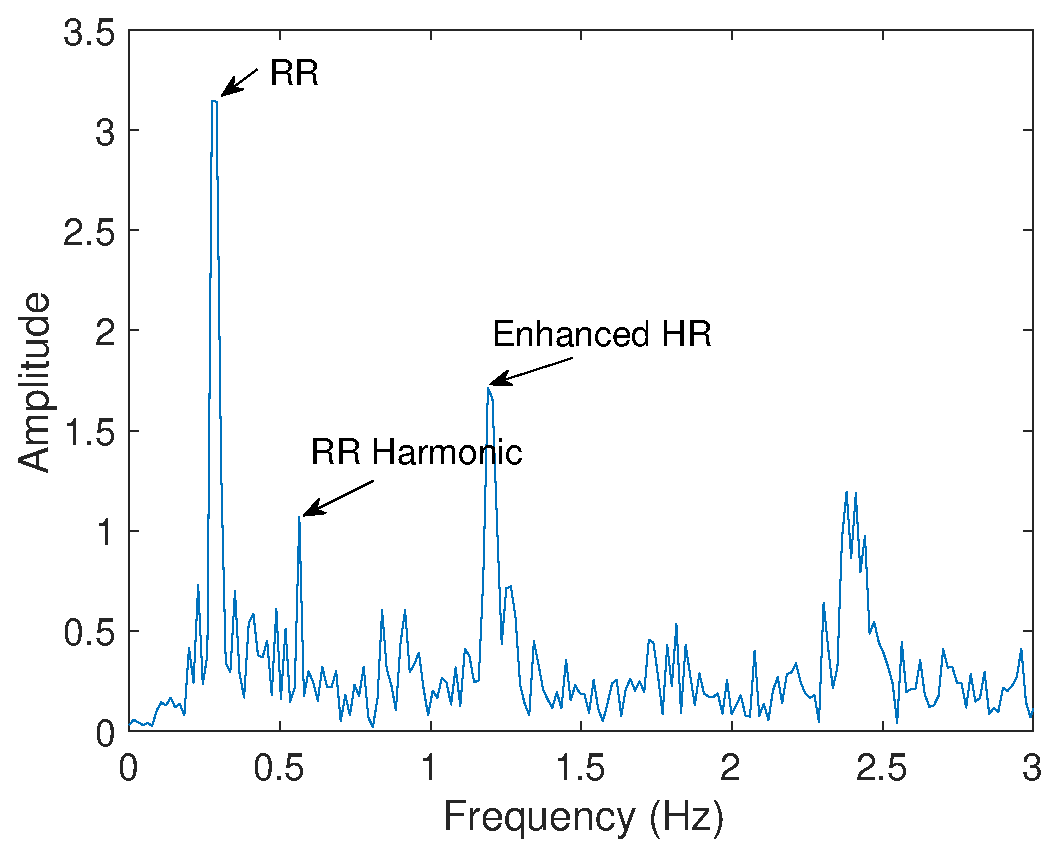
\includegraphics[width=0.25\columnwidth]{fftForHR_diff.eps}} 
    \caption{Illustration for spectrum-based methods: (a) raw radar signal; (b) spectrum obtained for raw radar signal from FFT, with RR, RR harmonic and HR peaks labelled; (c) raw radar signal after differentiation; (d) spectrum obtained for differentiated raw radar signal from FFT, with enhanced HR peak labelled.}
    \label{fig:fftForHR}
\end{figure}

\subsubsection*{Evaluations}
The spectrum-based methods are matured in the signal-processing area and can be implemented directly on the hardware with limited computational resources while achieving good real-time performance~\cite{hu2014real,park2017polyphase}. In fact, several commercial data-capture boards for raw radar signal processing have already embedded these algorithms on \gls{fpga}~\cite{obadi2021survey}. For the disadvantages, the spectrum-based methods are not sensitive to the abrupt HRV, because multiple cardiac cycles are involved in a single segment truncated by the time window, but only one HR value can be estimated from each segment~\cite{shi2021contactless}. Another problem caused by the truncation is that each segment may not contain integral multiples of the cardiac cycles, causing the shift of the estimated HR around the true HR~\cite{ye2018stochastic}. Lastly, various noises (such as RR harmonics and slight RBM~\cite{yamamoto2018spectrogram}) may have the frequency components falling into the HR frequency band and hence dominate the HR components~\cite{rong2019remote}. Although it is possible to extract the cardiac features using HR harmonics from the high-frequency spectrum (e.g., $1.5-5$ Hz) to avoid the effect of strong RR harmonic components~\cite{le2019multivariate}, the HR harmonics sometimes might be too weak and easily distorted by unexpected noises (e.g., car vibrations~\cite{da2019theoretical}).

\subsection{Periodicity-based Methods}
Periodicity-based methods are based on the natural periodicity of the cardiac features and leverage probability model (e.g., hidden Markov model)~\cite{kim2019peak, zhang2020health, mogi2017heartbeat, yamamoto2018spectrogram, xu2021accurate, ye2021spectral, will2018radar, wang2020remote, nosrati2017high, ha2021wistress, will2016instantaneous, lv2018doppler, ha2020contactless, zhao2016emotion, chen2022contactless, will2017advanced, sakamoto2015feature, xia2021radar, mei2020fast, will2018radar, shi2021contactless}, auto/cross-correlation~\cite{shi2021contactless} or template determined by cardiac morphology~\cite{will2017advanced} to identify the periodical patterns obscured by noise in radar signals~\cite{sakamoto2015feature}. This type of methods could identify a single heartbeat by either measuring the similarity between template and raw signals or predicting the next heartbeat based on a probabilistic model. In addition, periodicity-based methods further enable the fine cardiac event segmentation which is valuable for clinical diagnosis~\cite{ha2020contactless}. Lastly, periodicity-based methods are naturally immune to the noises that do not show any periodic feature.

\subsubsection*{Evaluations}
The above mentioned advantages of periodicity-based methods rely on certain prior knowledge (e.g., \gls{ppi} or ECG waveform) to design the template/model, but such template/model may be unsuitable for the monitoring of new participants and hence require certain calibration during actual monitoring~\cite{gong2021rf}. Furthermore, the optimal template/model with periodicity features learned from datasets may not fit the diverse cardiac features of other individuals~\cite{zhang2020health}. In other words, the researchers need to balance the ability to detect rare cardiac events (e.g., heart diseases) against the ability to provide accurate HR estimations for most scenarios.

\subsection{Blind Source Separation Methods}
\Gls{bss}  is a classic problem originally in the audio processing field to separate a group of signals (e.g., voices of different people) from the mixed signal received by microphone(s)~\cite{cardoso1998blind}. For radar-based cardiac monitoring, the received signal is also a nonlinear mixing of various sources such as RR, RBM, cardiac vibration and multi-path interference~\cite{lee2016tracking, bechet2013non, yamamoto2018non, mercuri2018direct,yamamoto2019music, ye2019blind,mercuri2021enabling, xu2021accurate, lv2021non, liu2020vital, diraco2017radar, zhang2020health, sun2020remote, shyu2018detection, shyu2020uwb, shen2018respiration, duan2018non, zhang2021mutual, wang2021mmhrv, wang2019noncontact, ye2018robust, ye2018stochastic}. The methods introduced in this subsection aim to decompose the mixed signal and extract the cardiac vibration signal according to different criteria:
\begin{itemize}
    \item \Gls{music}: orthogonal signal spaces for cardiac signal and noises;
    \item \Gls{ica}: statistical independence between cardiac signal and noises;
    \item \Gls{emd}: time-scale features in mixed signals;
    \item \Gls{vmd} and \gls{ssr}: natural sparsity of heartbeats.
\end{itemize}

\subsubsection*{Evaluations}
BSS methods do not require prior knowledge regarding cardiac events and can decompose the mixed signal according to specific characteristics. In addition, instead of modelling the heartbeat signal as a summation of a finite number of periodic sinusoidal signals~\cite{shen2018respiration}, most BSS methods assume that the source signals are not simple sinusoidal functions but with narrow bandwidth, enabling the non-linear decomposition of the mixed signal.

For the drawbacks, an ideal decomposition result relies on the careful selection of the parameters (e.g., $P$ for MUSIC, WGN for EMD, $K$ for VMD), whereas these parameters are obtained empirically and require a re-selection after altering the monitoring environment. The inappropriate selection of parameters can cause the mode mixing or over-decomposition issue, making it impossible to extract HR from the decomposed signals~\cite{weishaupt2018vital}. Lastly, it is still a challenge to select the proper decomposed signals for HR estimation because there are multiple decomposed signals falling into the heartbeat frequency band~\cite{shyu2018detection}.

\subsection{Deep Learning Method}
Deep learning belongs to machine learning based on artificial neural networks, but has multiple hidden layers formed by numerous neurons to achieve great performance. Each neuron receives a set of weighted inputs from other neurons and outputs the result through an activation function to introduce the non-linearity into the deep learning model~\cite{ha2020contactless, chen2021movi, chen2022contactless, wu2019person, yamamoto2020ecg, gong2021rf, shi2021contactless, li2019standalone, ye2021spectral}. Normally, the deep learning models with multiple hidden layers require complex structures and training methods, but are suitable for modelling the complex cardiac monitoring problem because the target signals are non-linearly modulated with other noises~\cite{chen2021movi}. In addition, to enable the deep learning model to learn the latent information (high-level features) buried in the signal, a massive amount of data mostly needs to be fed into the deep learning model to find the optimal weights after iterative training.
. 

In the literature, radar-based ECG waveform recovery has been achieved based on various deep-learning architectures, such as \gls{cnn})~\cite{chen2022contactless,zhang2024radarODE}, \gls{lstm} network~\cite{ji2022rbhhm}, and Transformer~\cite{chen2022contactless,wu2023contactless}. However, the noise robustness of the deep-learning framework is rarely investigated in the literature, especially for the RBM noise that is inevitable in contactless monitoring and has orders of magnitude larger than cardiac activities. The existing work either discarded the data during the RBM~\cite{wang2023ecg} or reported the heavy distortion as the future work~\cite{chen2022contactless}. Additionally, the existing deep-learning methods are also blamed for being purely data-drove as a black box and the transformation between cardiac mechanical and electrical activities lacks the theoretical explanation~\cite{zhang2024radarODE}. 

\subsubsection*{Evaluations}
Due to the powerful fitting capability of the deep learning model, deep learning methods can model complex and non-linear projections and hence produce fine-grained cardiac signals (e.g., ECG) compared with the algorithms in other categories. In addition, with a special network design (e.g., LSTM network), the deep learning model can memorize long-term dependency from the dataset, making stable long-term cardiac monitoring possible. Lastly, compared with the other three categories of methods, the deep learning methods can potentially resist different kinds of noises by introducing these noises during the dataset collection~\cite{chen2021movi}.

The outstanding performance of deep learning methods generally relies on the training with a large-scale and full-featured dataset~\cite{schellenberger2020dataset}, whereas the well-trained deep learning model may fail to infer on the data out of distribution~\cite{gong2021rf}. For example, the deep learning model trained on the dataset for normal people cannot perform accurate cardiac monitoring for patients with different cardiac features. Similarly, the deep learning model trained on the dataset collected for multi-path effect mitigation cannot resist the RBM noise. Therefore, the collected dataset should contain various real-world scenarios, increasing the complexity of establishing a full-featured dataset. Additionally, it is still a challenge to implement complex deep learning models on compact and lightweight devices with real-time monitoring ability, because effective deep learning models normally require ample computational resources and large memory.